\apendice{Anexo de sostenibilización curricular}

\section{Introducción}

Durante el desarrollo del Trabajo de Fin de Grado, se han podido incluir diferentes aspectos relacionados con el desarrollo sostenible, no limitándose únicamente a los aspectos medioambientales, sino también a los sociales y económicos. La sostenibilidad ha sido un aspecto transversal en el proyecto, presente desde el diseño hasta la implementación del proyecto, considerando tanto el impacto inmediato como el impacto a largo plazo de las decisiones tomadas. 

Es importante destacar los 17 objetivos de desarrollo sostenible(ODS) propuestos por las Naciones Unidas\footnote{Naciones Unidas. \textit{Objetivos de desarrollo sostenible}. \url{https://www.un.org/sustainabledevelopment/es/objetivos-de-desarrollo-sostenible/}}. Estos objetivos formar una hoja de ruta para abordar los  retos globales y que abarcan desde la acción por el clima, la igualdad de género, la educación, la salud y el bienestar entre otros.

En el contexto de este proyecto, se han tenido especialmente en cuenta los siguientes ODS:

\begin{itemize}
    \item \textbf{ODS 7: Energía asequible y no contaminante}, mediante la utilización de servicios en la nube comprometidos con energías renovables y los objetivos de desarrollo sostenible.
    \item \textbf{ODS 9: Industria, innovación e infraestructura}, promoviendo el uso de tecnologías innovadoras y fácilmente escalables, como son la inteligencia artificial y el diseño modular.
    \item \textbf{ODS 12: Producción y consumo responsables}, a través de la optimización y el uso eficiente de recursos.
    \item \textbf{ODS 13: Acción por el clima}, reduciendo el impacto ambiental mediante la eficiencia energética y la selección de proveedores de servicios comprometidos.
    \item \textbf{ODS 17: Alianzas para lograr los objetivos}, con el uso de tecnologías de código abierto permite un mayor avance.
    \item \textbf{ODS 4: Educación de calidad} y \textbf{ODS 10: Reducción de las desigualdades}, facilitando el acceso a la web a todo el mundo y disponible en varios idiomas.
\end{itemize}



En primer lugar, se ha tenido en cuenta el impacto medioambiental de las tecnologías utilizadas, como el uso de contenedores Docker para la ejecución del proyecto. Esta tecnología permite una mayor eficiencia en el uso de recursos, incluyendo una mayor capa de seguridad y facilitando la escalabilidad de la aplicación, lo que contribuye a una reducción del consumo energético y de utilización de recursos. También se han utilizado servicios de terceros en la nube, comprometidos con la sostenibilidad, como es el caso de GitHub~\cite{SosGithub}, Cloudflare~\cite{SosCloudflare} y AWS~\cite{SosAWS}.

\section{Uso sostenible de recursos}

Uno de los aspectos más relevantes del proyecto es el uso eficiente de los recursos y la optimización de los mismos. Para ello, se han implementado diversas estrategias que permiten reducir el consumo de recursos y minimizar el impacto ambiental.

En primer lugar, se ha optado por el uso de Cloudflare como proveedor de servicios de DNS y CDN, lo que permite mejorar las velocidades de carga, disminuyendo el ancho de banda y consultas al servidor de origen, ahorrando tiempo de cómputo. Cloudflare también se compromete con la sostenibilidad y ha implementado diversas iniciativas para reducir su huella de carbono, como el uso de energías renovables en sus centros de datos~\cite{SosCloudflare}. Cloudflare proporciona un informe sobre el impacto de carbono de los servicios usados, aunque no se ha podido obtener el informe para este proyecto en concreto, ya que no se ha alcanzado el umbral mínimo de uso de recursos para que se genere dicho informe. Aunque una de las métricas que sí se pueden obtener es el número del ancho de banda ahorrado, que en este caso se muestra en la \textbf{Figura~\ref{fig:ancho}}.

\begin{figure}[!h]
    \centering
    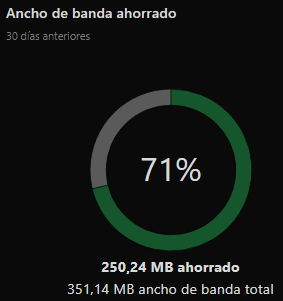
\includegraphics[width=0.4\textwidth]{ancho}
    \caption{Ancho de banda ahorrado por el uso Cloudflare}\label{fig:ancho}
\end{figure}
\FloatBarrier

En la \textbf{Figura~\ref{fig:ancho}} se puede observar que se ha ahorrado un porcentaje considerable, que se traduce en un menor tiempo de cómputo, que deriva en una reducción del consumo energético, del impacto ambiental y reducciones de costes.

Además, se ha elegido un diseño de aplicación modular y escalable, que permite una fácil adaptación a futuros cambios y mejoras, así como una mejor gestión de los recursos individuales de cada módulo.

\section{Uso de tecnologías de código abierto}
El proyecto ha utilizado en su mayoría tecnologías de código abierto, que permiten una mayor sostenibilidad del proyecto, ya que promueven la transparencia, la colaboración, la auditabilidad del código y el acceso equitativo a la tecnología.~\cite{SosOpen}. Además, se permite contribuir al proyecto de forma abierta, facilitando la mejora continua del mismo y la posibilidad de mejorar el soporte a la comunidad, ya que se pueden realizar auditorías de seguridad y mejoras en el código por parte de la comunidad.


\section{Consideraciones sobre la sostenibilidad social y económica}
En los aspectos sociales y económicos, se ha tenido en cuenta la importancia de la accesibilidad y la inclusión en el desarrollo del proyecto. Por ejemplo, en la parte de la web se ha implementado un sistema de localización que permite que la aplicación sea accesible a un público más amplio, en el que de momento está disponible en español e inglés, pero se puede ampliar a otras regiones fácilmente. Además, se ha añadido la opción de cambiar el tema de la aplicación, para que sea más accesible a las personas, en el que se puede cambiar entre un tema claro y oscuro, para adaptarse a las preferencias del usuario y mejorar la experiencia de uso.


\section{Conclusiones}
En resumen, el proyecto ha tenido en cuenta diversos aspectos relacionados con la sostenibilidad, tanto medioambientales como sociales y económicos. Se han implementado diversas estrategias para reducir el impacto ambiental, optimizar el uso de recursos y promover la accesibilidad y la inclusión, como son el uso de tecnologías de código abierto y el uso de servicios de terceros comprometidos con la sostenibilidad.